        \clearpage
        \begin{figure*}[ht]
            \pdfbookmark[2]{ID 05}{figure_id_05}
        	\centering
            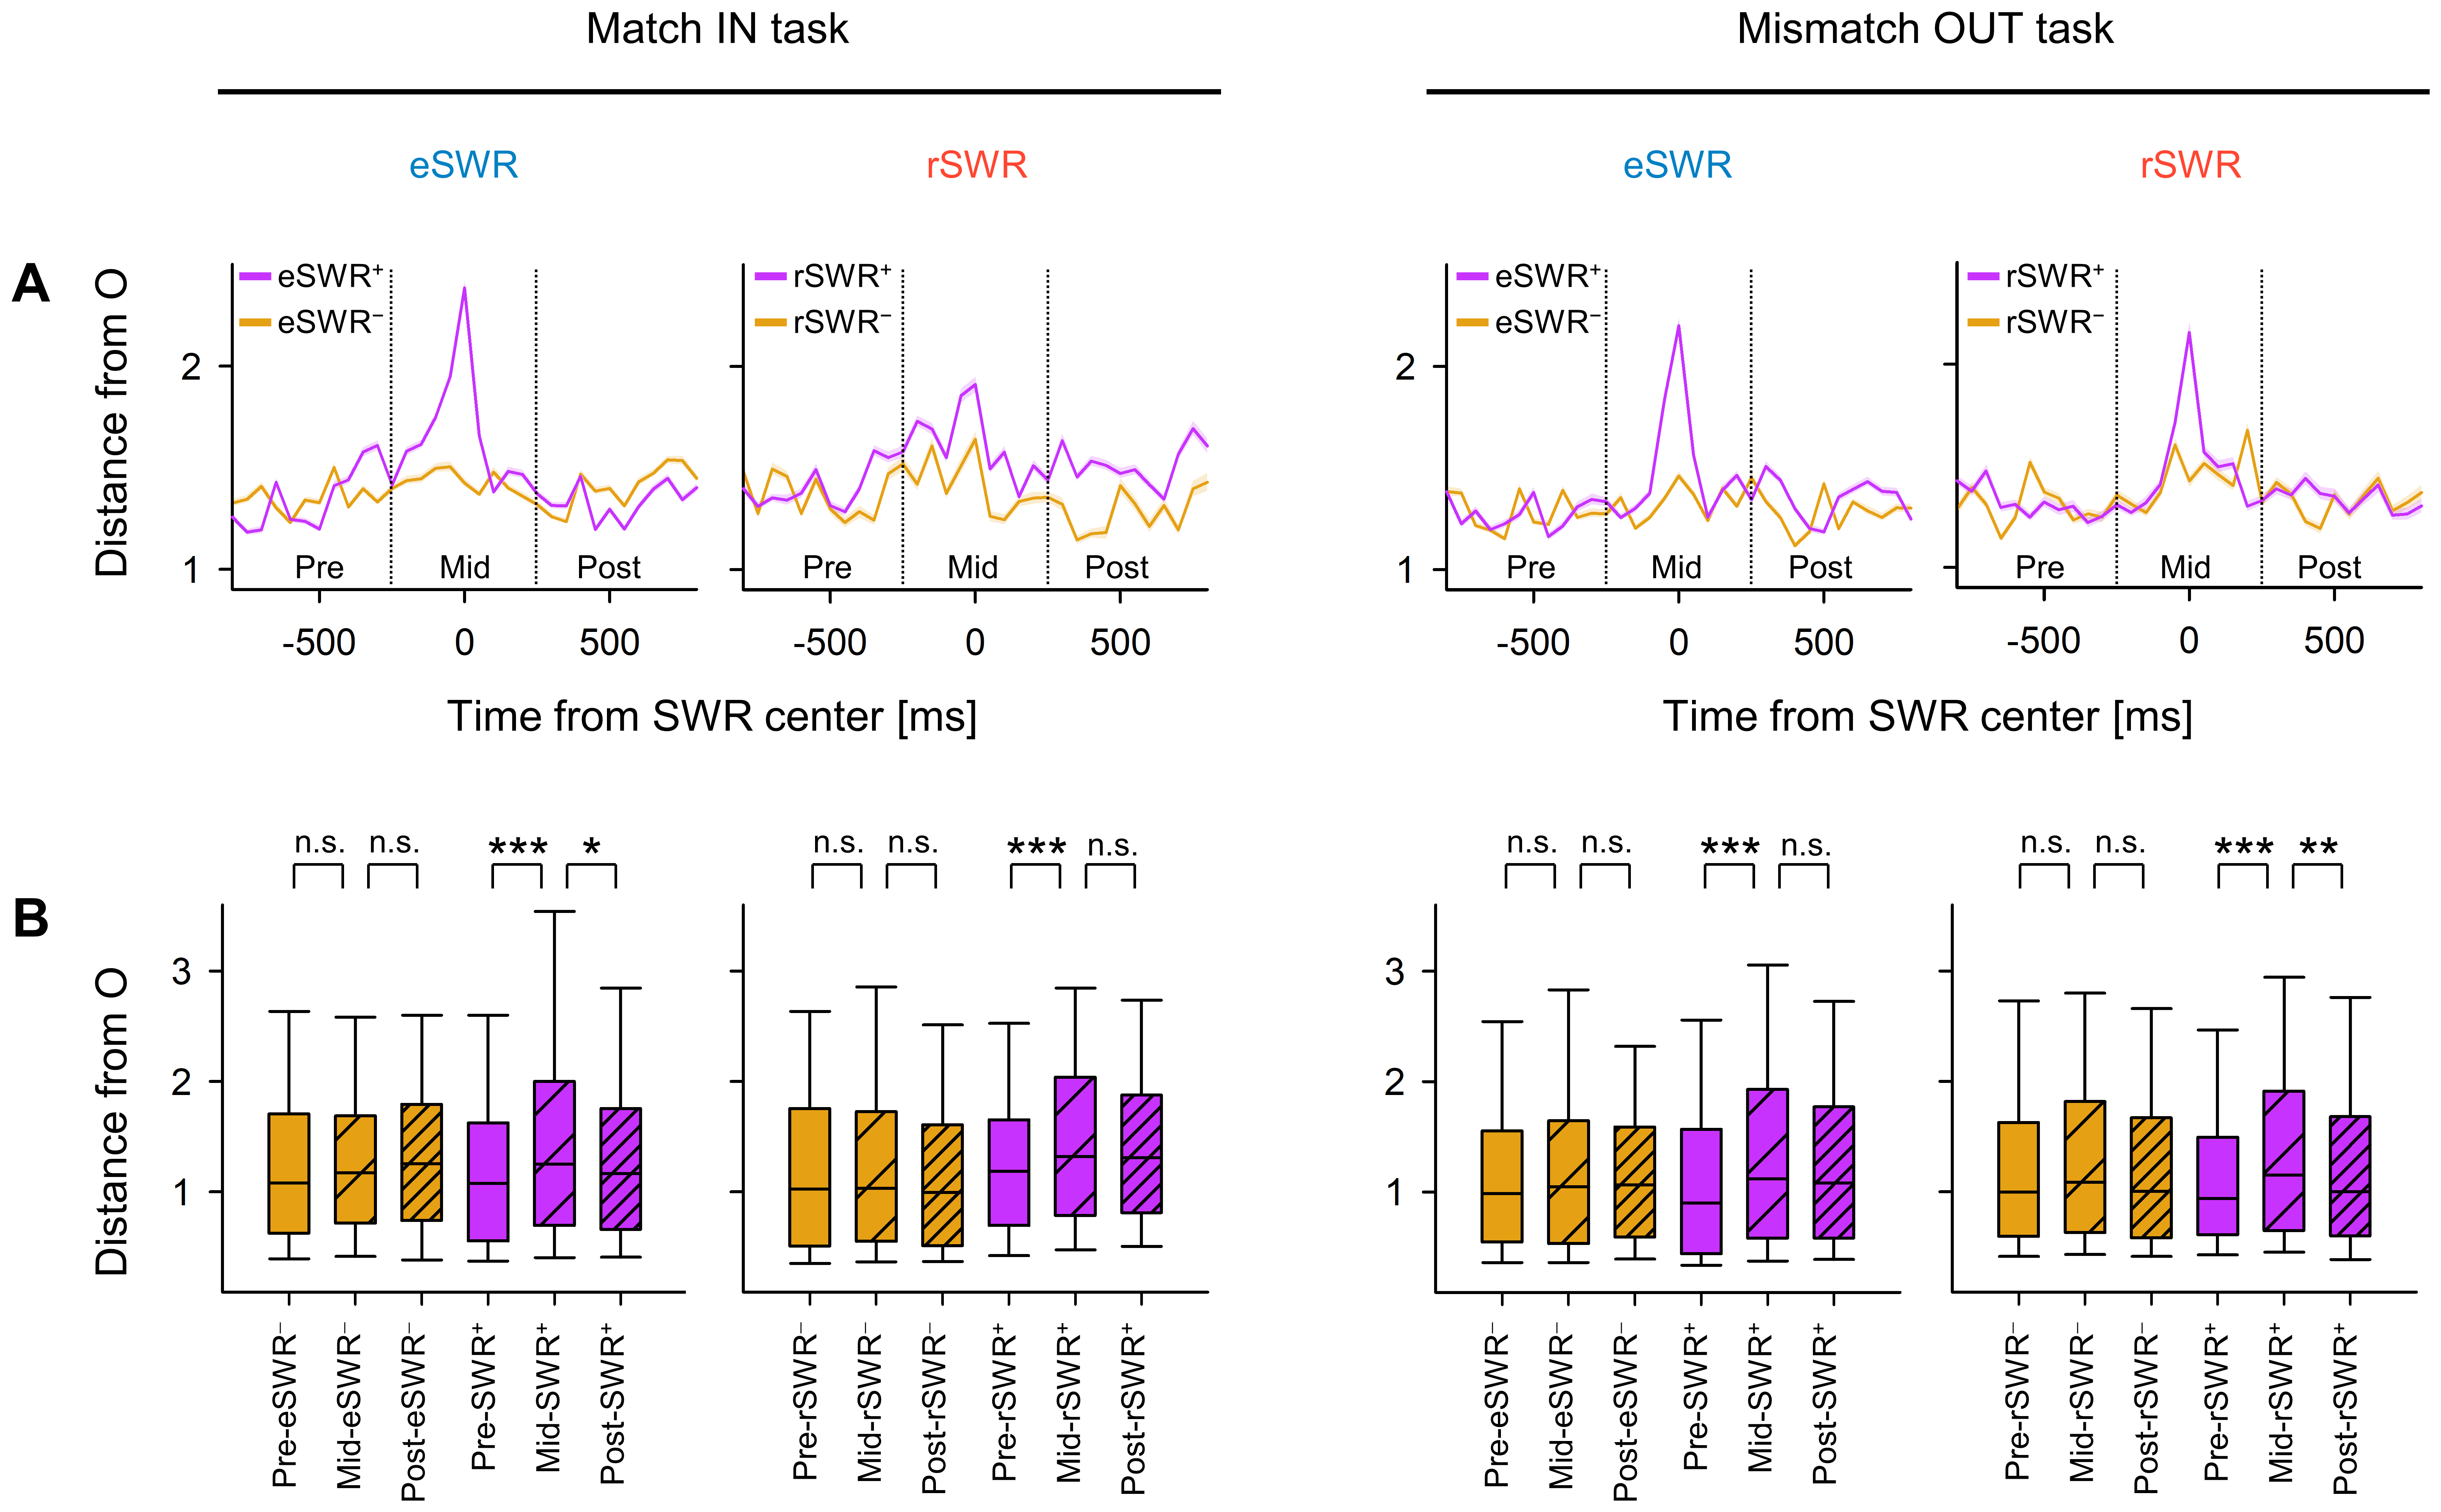
\includegraphics[width=1\textwidth]{./src/figures/.png/Figure_ID_05.png}
        	\caption{\textbf{Transient Alterations in Neural Trajectory During SWR}
\smallskip
\\
\textbf{\textit{A.}} Indicates the mean distance from the origin ($O$) of the peri-sharp-wave-ripple (SWR) trajectory, which is accompanied by a 95\% confidence interval that may not be visually detectable due to its narrow range \cite{girardeau_selective_2009,norman_hippocampal_2019,buzsaki_hippocampal_2015}. \textbf{\textit{B.}} Depicts the distance from the origin ($O$) during the pre-, mid-, and post-SWR periods (*\textit{p} $<$ 0.05, **\textit{p} $<$ 0.01, ***\textit{p} $<$ 0.001; per the Brunner--Munzel test \cite{boran_persistent_2019}). Definitions included are: SWR, sharp-wave ripple events; eSWR, SWR occurring during the encoding phase; rSWR, SWR transpiring in the retrieval phase; SWR$^+$, a SWR event; SWR$^-$, the control events paired with SWR$^+$; pre-, mid-, or post-SWR, the time intervals from $-800$ to $-250$ ms, from $-250$ to $+250$ ms, and from $+250$ to $+800$ ms, respectively, each relative to the SWR center.
}
% width=1\textwidth
        	\label{fig:05}
        \end{figure*}
